\documentclass[12pt]{article}
\pagestyle{headings}
\usepackage{amssymb}
\usepackage{amsmath}
\usepackage[czech]{babel}
%\usepackage[utf8]{inputenc}
\usepackage{fancyhdr}

\usepackage{graphicx}
\graphicspath{ {./img/} }

\DeclareMathAlphabet{\mathcal}{OMS}{cmsy}{m}{n}
\SetMathAlphabet{\mathcal}{bold}{OMS}{cmsy}{b}{n}
\newcommand{\bigO}{\mathcal{O}}
\newcommand{\bigOlog}{\bigO(\log(n))}


\title {Data Structures I notes}
\author {Kyrylo Karlov}
\date {\today}

\begin {document}

\maketitle
\tableofcontents

\pagebreak

\section{Basic DS}

Popište „nafukovací pole“ se zvětšováním a zmenšováním. Analyzujte jeho amortizovanou složitost.


\section{Search trees}
A group of DS that supports fast Lookup.


\subsection{BB[alpha] tree}
An example of locally lazy rebuild DS.

A tree is perfectly balanced if
\[ \forall v \in V : | s(l(v) - s(r(v)) | = 1 \]
Meaning for each node left and right subtree sizes are almost equal, 1:1 ratio.

However maintaining perfectly balanced tree requires $ \bigO(n) $, therefore we would use ratio between 2:1 and 1:2.
\paragraph{Def:} A node w is in balance if

\[ \forall v \in T(w) : s(v) \leq 2/3 * s(w) \]

A tree is balanced if every node is balanced.

\subsubsection{Time and space complexity}
Popište BB[alpha]-stromy s líným vyvažováním. Analyzujte jejich amortizovanou složitost.

\paragraph{Find} Height of a balanced tree with n nodes is $ \bigO(\log(n)) $.
Take an arbitrary path from the root to a leaf. Root has size n, each subsequent node has at most 2/3 of parent's size. Leaf has size 1. Therefore the path contain at most $ \log_{2/3} (1/n) = \log_{3/2}(n) = \bigO(\log(n)) $ edges. So lookup is also $ \bigO(\log(n)) $ .

\paragraph{Insert} Along the path we check that nodes are in balance. If they are, we are done. Otherwise take highest out-of-balance node w and rebuild T(w) to make it perfectly balanced, which takes $ \bigO(s(w)) $.

\paragraph{Theorem} Amortized time complexity of Insert is $ \bigO(\log(n)) $.
We define potential (how far is current tree from perfectly balanced):
\[ \Phi =  \sum_{v \in V} \varphi(v)\]
\[ \varphi :=
	\begin{cases}
		|  s(l(v) - s(r(v)) | &\quad\text{if at least 2} \\
		\text {0} &\quad\text{otherwise}
	\end{cases}
\]

After Insert, the contribution of new vertices will increase by 2 max, because of definition it can jump from 0 to 2.

No rebuild - we spent $ \bigO(\log(n)) $ on operation itself and potential is increased by $ 2*\log(n) $ max, therefor total amotrized cost is $ \bigO(\log(n)) $.

Otherwise we should rebuild at node w. WLOG the invariant is broken for w and its left child c. So
\[ s(l(w)) < 2/3 * s(w) \]
and the other subtree has
\[ s(r(w)) < 1/3 * s(w) \]
the contribution of w is
\[ \varphi(w) > 1/3 * s(w) \]

After the reubild, $ \varphi(w) = 0 $ as well as all nodes in subtree. All other potentials are the same. The whole potential is decreased by at least $ 1/3 * s(w) $. The real cost of rebuild is $ \bigO(s(w)) $. After multiplying the potential after a suitable constant the real cost would be offset by the change in potential, yielding zero zmortized cost of the rebuild. TODO ???

\paragraph{Delete} TODO


\subsection{Splay tree}

Self-adjusting binary search trees. Heuristics: bring the lowest accessed node to the top during every operation. Double rotations are used instead of single.
Such heuristics guarantee amortized $\bigO(n\log(n))$ cost of all operations.

\paragraph{Splay}
Splay operation - brings node to the top using double and single rotations.

\paragraph{Theorem:} The amortized cost of Splay(x) is at most $ 3 (r'(x) - r(x)) + 1 $ where r(x) is rank before and r'(x) is after Splay.

Let r(v) be binary log(s(v)) a rank of w.

Total cost is a sum of individual steps. Let $ r_1(x), ..., r_t(x) $ is a rank of x after each step, initial is $ r_0(x) $.
The amortized cost of the i-th step is at most $ 3 (r_i(x) - r_{i-1}(x)) $

\paragraph{Helper lemma:}
$ log(\frac{a + b}{2}) \geq \frac{log(a) + log(b)}{2} $. Inequality is true for all concave functions.

\paragraph{Corollary:} $ log(a) + log(b) \leq 2log(a + b) - 2 $.

\subsubsection*{Zig-zag}
The real cost of the operation is 2. Let the tree be y -left w -right x. Then potential increases by:
\[ \delta = (r'(w) - r(w)) + (r'(x) - r(x)) + (r'(y) - r(y)) \]

The amortized cost is:
\[ A = 2 + \delta \]

using the Corrolary:
\[ r'(w) + r'(y) = log(s'(w)) + log(s'(y)) \leq 2log(s'(w) + s'(y)) - 2 \]

The subtrees T'(w) and T'(y) are disjoint and they are contained in T'(x), so we have
\[log(s'(w) + s'(y)) \leq log s'(x) = r'(x)\].
Thus:
\[ r'(w) + r'(y) \leq 2r'(x) - 2 \]
Substituting this to the inequality for A yields:
\[ A \leq 3r'(x) - r(w) - r(x) - r(y) \]
Also
\[ r(w) \geq r(x) \land r(y) \geq r(x) \]
Total

\[ A \leq 3(r'(x) - r(x)) \]

\subsubsection*{Zig-zig}
Similar to Zig-Zag.
\[ A = 2 + \delta \]
The subtrees T(x) and T'(z) are disjoint, so using the Corrolary:
\[ r(x) + r'(z) = log(s(x)) + log(s'(z)) \leq 2log(s(x) + s'(z)) - 2 \leq 2log(s'(x)) = 2r'(x) - 2 \]
Or
\[ r'(z) \leq 2r'(x) - r(x) - 2 \]
So
\[ A \leq 3r'(x) + r'(y) - 2r(x) - r(y) - r(z) \]
\[ T(z) = T'(x) \implies r(z) = r'(x) \]
\[ T(y) \supseteq T(x) \implies r(y) \geq r(x) \]
\[ T'(y) \subseteq T'(x) \implies r'(y) \leq r'(x) \]
Total

\[ A \leq 3(r'(x) - r(x)) \]

\subsubsection*{Zig}

\[ A = 2 + (r'(x) - r(x)) + (r'(y) - r(y)) \]
By inclusion of subtrees, we have $ r'(y) \leq r'(x) $ and $ r(y) \geq r(x) $, hence:
\[ A \leq 1 + 2r'(x) - 2r(x) \]
as $ r'(x) - r(x) > 0 $
\[ A \leq 1 + 3r'(x) - 3r(x) \]

\subsubsection{Time and space complexity}

Navrhněte operace Find, Insert a Delete na Splay stromu. Analyzujte jejich amortizovanou složitost.

\paragraph{Find}
1. Find (x) as in binary tree \\
2. Splay (x) or the last accessed node

Either successfull of successfull FIND stops at some node at depth d. Then we splay this node.
Going from Root costs $ \Theta(d) $ and does not change the potential. Splay will cost $ \Theta(d) $ and amortizes to $\bigO(\log(n))$. Adding going from root to Splay cost which results in multiplying by the constant both amortizing cost and potential. In total whole FIND is $\bigO(\log(n))$.

\paragraph{Insert}

1. Find (x) as in binary tree \\
2. If already present - Splay(x) and the time complexity is the same as FIND
3. Else - add leaf and Splay(x)

Adding leaf is constant, so besides the potential change time complexity is the same as FIND.

\paragraph{Lemma} Adding leaf increases potential by $\bigO(\log(n))$.
Let $ r(v_1), ... , r(v_{t+1}) $ are potentials on the path from root to new leaf (t + 1). The potential change is
\[ \Delta \Phi = r'(v_{t+1} + \sum_{i = 1}^t (r'(v_i) - r(v_i)) \]
as newly added node is leaf:
\[ r'(v_{t+1} = 0 \]
Other potentials increase by 1, also
\[ r'(v_i) \leq r(v_{i - 1}) \]
as the sum is telescopic
\[ \Delta \Phi \leq r'(v_1) - r(v_1) \]
Which is $\bigOlog$.

\paragraph{Delete}

1. Find(x)
2. Delete(x)
	a. x is a leaf
	b. x has 1 child
	c. x has 2 children - replace x by min in R subtree. Reduces to b.

The cost of walking to the node (FIND) is offset by splaying parent of the removed node. If node has no parent - node has constant depth and time complexity is constant.

Removing a node has constant real cost. The change in the potential is in favor of us: we are removing one node from the potential and decreasing the ranks of all its ancestors, so the potential difference is negative.
We can conclude that Delete runs in $\bigOlog$ amortized time.

\subsection{A-B tree}
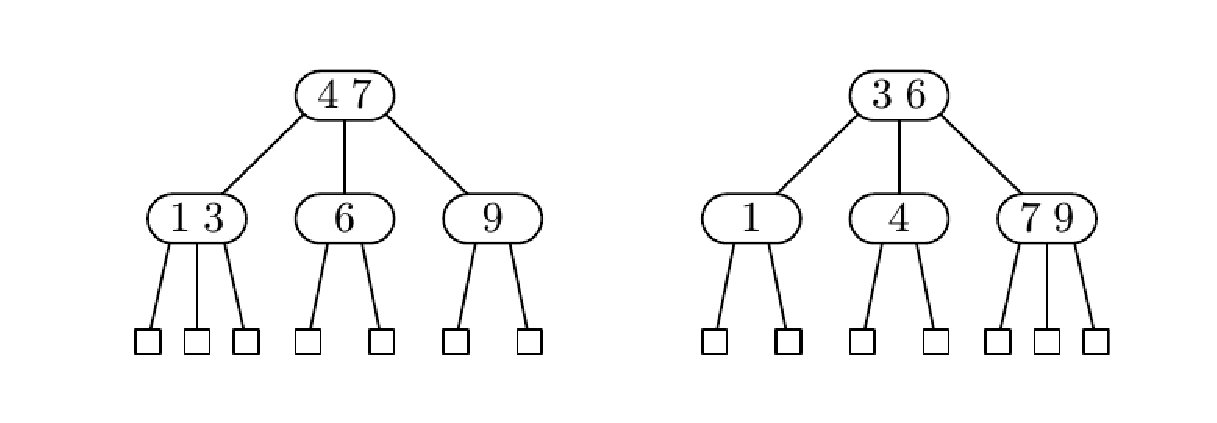
\includegraphics[scale=0.5]{a_b_tree}

Definition: An (a,b)-tree for parameters $a \geq 2$ and $b \geq 2a - 1$ is a multi-way search tree, which satisfies:

1. The root has between 2 and b children (unless it is a leaf, which happens when the set of keys is empty). Every other internal node has between a and b children. \\
2. All external nodes have the same depth.

\paragraph{Lemma:} The height of an (a, b)-tree with n keys $  \log_b(n + 1) \leq h \leq 1 + \log_a ((n + 1)/2)$.

The min number of keys in tree with height h. On Level 0 only root with 1 key. Level h contains only external nodes. The i-th level in between has $2a^{i-1}$ nodes with a-1 keys each. So
\[ 1 + \sum_{i=1}^{h-1} 2a^{i-1} = 1 + 2(a-1) \sum_{i=1}^{h-2} a^i = 1 + 2(a-1) \frac{a^{h-1} - 1}{a-1} = 2a^{h-1} - 1 \]
So
\[ n \geq 2a^{h-1} - 1 \implies h \leq 1 + \log_a ((n + 1)/2) \]

The max keys in tree of height h. All levels will have $b^i$ nodes at level i, each with (b-1) keys. In total:
\[ \sum_{i=0}^{h-1} b^i(b-1) = (b-1) \sum_{i=0}^{h-1} b^i = (b-1) * \frac{b^h - 1}{b-1} = b^h - 1 \]
So
\[ n \leq b^h - 1 \implies h \geq \log_b(n + 1) \]
\parahraph{Corollary:} The height is $\Omega(\log_b n)$ and $\bigO(\log_a n)$.


\subsubsection{Time and space complexity}

    Definujte (a,b)-strom. Popište, jak na něm probíhají operace Find, Insert a Delete. Rozeberte jejich slozitost v nejhorším případě.

\paragraph{Find} $\bigO(\frac{log(b)}{log(a)}*log(n))$
\paragraph{Insert}  $\bigO(\frac{b}{log(a)}*log(n))$
\paragraph{Delete} $\bigO(\frac{b}{log(a)}*log(n))$

\subsubsection{Amortized Time complexity for (a, 2a-1) and (a, 2a) }
From the Time complexity of operations we want smallest b. Ideally b = 2a, b = 2a - 1 is worse.

In an amortized sense, (a, b)-trees cannot perform better than in $\Omega(log(n))$, because all operations involve search, which can take $\bigO(log(n))$ repeatedly.

\paragraph{Theorem:} A sequence of m Inserts on an initially empty (a, b)-tree performs $\bigO(m)$ node modifications.
Number of splits $ \#s \leq \# $ of inner nodes at the end $ \leq m$.

When we start mixing insertions with deletions, the situation becomes more complicated.
In a (a, 2a - 1)-tree, it might happen that Insert(x) forces splitting up to the root and
the immediately following Delete(x) undoes all the work and reverts the tree back to the original state. So we can construct an arbitrarily long sequence of operations which have $\Omega(log(n))$ cost each.
DS oscilates between 2 states. Therefore modification amortized time cannot be constant.

When we increase b to at least 2a, it is sufficient to avoid oscillations and keep the amortized number of changes constant.
For simplicity, we will prove this for the specific case b = 2a.

\paragraph{Theorem:} A sequence of m Inserts and Deletes on an initially empty (a, 2a)-tree performs O(m) node modifications.
Define potential, so that Insert, Delete and Rotation will be $\bigO(1)$ but operations Slit, Merge will have negative potential.
\[ \Delta \Phi = \sum_{v} f(|v|)  \]
with
\[ f:\{ a-2, ..., 2a \} < 0 \]

The function fshould satisfy the following requirements:
1. $|f (i) - f (i + 1)| \leq c$ for some constant c. \\

This means that if the number of keys in the node changes by 1, the node’s contribution changes at most by a constant.

2. $f(2a) \geq f(a) + f(a - 1) + c + 1$.
This guarantees free splits. TODO desc

3. $f(a - 2) + f(a - 1) \geq f(2a - 2) + c + 1$.
This guarantees free merges. TODO desc

Such function is c = 2 and
\[ f(a-2) = 2 \land f(a-1) = 1) \]
and
\[ f:{a, ..., 2a-2} = 0 \]
Finally
\[ f(2a-1) = 2 \land f(2a) = 4) \]

Insert and Delete are amortized constant. After m operations we woudld get
\[ \bigO(m) + \Phi_m - \Phi_0 = \bigO(m) \]
as $ \Phi_m \geq 0 \land \Phi_0 = 0 $ since tree was empty.

\section{Cache friednly DS}
\subsection{I/O complexity}
\subsection{K-way merge sort}
A K-way Mergesort combines K runs at once, so the number of passes decreases to $ \lceil \log_K N \rceil = \lceil log N/log K \rceil$ .
A K-way merge needs to locate a minimum of K items in every step, which can be done using a heap.
Every step therefore takes time $ \Theta(log K)$, so merging T items takes $\Theta(T log K) $ and the whole Mergesort $ \Theta(N log K * log N/ log K) = \Theta(N log N )$ for any K.

If cache is large enough, then every input array has its own scan and the heap fits the cache. Then total I/O complexity is $ \bigO(T/B + K)$. The extra K is required for situation when each run is located in different block (small runs). Which will never happen in Merge Sort (WHY???). Therefore total I/O complexity is $ \bigO(T/B + 1)$.

Each scan requires its own cache block, K + 1 blocks in total. Another  $K - 1$ for heap, so $M \geq 2BK$ is sufficient. If we know M and B $M = 2BK$. Then I/O complexity is $\bigO((N/B * log N)/log(M/B)+1)$.

\subsection{Matrix transpose}
Divide and Conquer algorithm. Try to aproximate tiles by recursive subdivisions. Let $N = 2^k$, then we can split matrix into 4 parts $A_{11}, A_{12}, A_{21}, A_{22}$. Quandrants $ A_{12}, A_{21} $ are divided into 4 TS (transpoze and swap) subproblems, diagonal are divided into 2 T (transpoze) and 2 TS subproblems (same as whole matrix).

Consider tree of recursion, every nide corresponds to a T or TS problem. It has 3 or 4 children for its sub-problems. At level i we have at most $ 4^i $ subproblems of size $ N/2^i $. Therefore the height of tree is log(N) and $ 4^{log(N)} = N^2 $ leaves.

In every TS leaf, we swap a pair of items. In every T leaf, nothing happens. Internal nodes only redistribute work and they do not touch items. So every node takes $ \bigO(1) $ time and the whole algorithm finishes in $ \bigO(N^2) $ steps.

To analyze I/O complexity, we focus on the highest level, at which the sub-problems correspond to tiles from the previous algorithm. Specifically, we will find the smallest i such that the sub-problem size $ d = N/2^i $ is at most B. Unless the whole input is small
and i = 0, this implies $ 2d = N/2^{i-1} > B$. Therefore $ B/2 < d \leq B$. Cache controller will use following optimal strategy: cache almost nothing before level i (recursion stack and local variables are asymptotically insignificant). At level i load whole subproblem into cache, which is equivalent to running cache-aware (tiles) algorithm for $ d \in \Theta(B) $ which requires $ \bigO(N^2/B) $ block transfers in total (is cache satisfies Tall-cache property).

For N different from powers of 2, some of the subproblems would be rectangular. However, sides differ by at most 1.  For almost-square matrices, our reasoning about the required number of block transfers still applies. Therefore we have reached optimal complexity $ \bigO(N^2/B + 1) $

\subsection{LRU cache model}

    Vyslovte a dokažte Sleatorovu-Tarjanovu větu o kompetitivnosti LRU.

\section{Hash DS}

\subsection{Bloome filters}
\subsubsection{1-line filter}
\subsubsection{k-line filter}

Let $ \varepsilon > 0 $, n is max \# of elements. For $ k = \lceil \log 1/\varepsilon \rceil $ a m = 2n. Then B. filter has probability of false positive $ < \varepsilon $.

\subsubsection{1-table filter}
Assume we have k independent absolutely random hash functions.

\subsubsection{Delete}

We cannot easily set bit in filter to 0 during delete, as we would lose false negative property. Therefore a helper counter array will be used.
At insert of delete we would increase/decrease counter. Then FIND will return true if $ C[h_i(x)] > 0 $. However, every item in array is limited to J bits and in case \[ C[i] = 2^J-1 \] it wouldnt increase any more (frozen). As a byproduct it will increase false positive results.

If there is too many frozen counters - rehash with new functions.

\paragraph{Analysis}

\section{Suffix arrays}

\end {document}
